
Given equation can be represented in a form as
\begin{equation}
\myvec{2 & -1 \\ 3 & 1}\myvec{x \\ y} = \myvec{10 \\ 5}
\end{equation}
The corresponding augmented matrix is 

\begin{align}
		\myvec{
		2 & -1 & \vrule & 10 \\
		3 & 1 & \vrule & 5 \\
	}
\end{align}

We use the Guass Jordan Elimination method as

\begin{align}
	\myvec{
		2 & -1 & \vrule & 10 \\
		3 & 1 & \vrule & 5 \\
	}
	\\
	\xleftrightarrow[]{R_2 \rightarrow R_2 - \frac{3}{2}R_1}
	\myvec{
		2 & -1 & \vrule & 10 \\
		0 & \frac{5}{2} & \vrule & -10 \\
	}
	\\
	\xleftrightarrow[]{R_2\rightarrow \frac{2}{5}R_2}
	\myvec{
		2 & -1 & \vrule & 10 \\
		0 & 1 & \vrule & -4 \\
	}
	\\
	\xleftrightarrow[]{R_1 \rightarrow R_1 + R_2}
	\myvec{
		2 & 0 & \vrule & 6 \\
		0 & 1 & \vrule & -4 \\
	}
	\\
	\xleftrightarrow[]{R_1 \rightarrow \frac{1}{2}R_1}
	\myvec{
		1 & 0 & \vrule & 3 \\
		0 & 1 & \vrule & -4 \\
	}
\end{align}

Therefore, the values of $x$ and $y$ are:

\begin{align}
	x = 3 \\
	y = -4
\end{align}
See Fig. \ref{aug/2/11/plt} for verification.
\begin{figure}[!h]
\centering
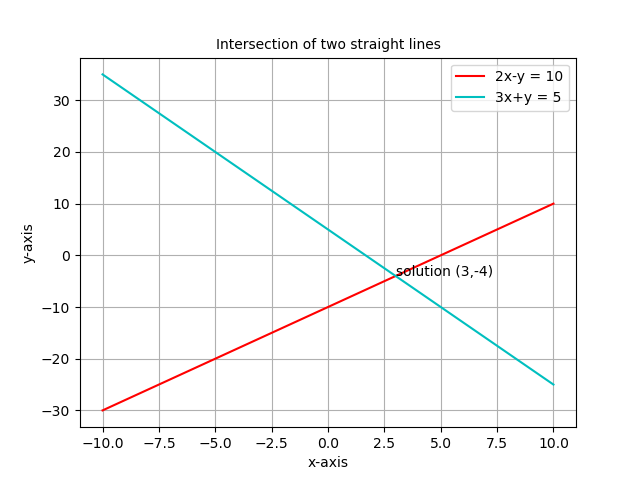
\includegraphics[width=\columnwidth]{solutions/aug/2/11/Figures/plot.png}
\caption{Plot of the line}
\label{aug/2/11/plt}
\end{figure}
